\documentclass[11pt,a4paper]{report}
\usepackage[textwidth=37em,vmargin=30mm]{geometry}
\usepackage{calc,xunicode,amsmath,amssymb,paralist,enumitem,tabu,booktabs,datetime2,xeCJK,xeCJKfntef,listings}
\usepackage{tocloft,fancyhdr,tcolorbox,xcolor,graphicx,eso-pic,xltxtra,xelatexemoji}

\newcommand{\envyear}[0]{2025}
\newcommand{\envdatestr}[0]{2025-02-19}
\newcommand{\envfinaldir}[0]{webdb/2025/20250219/final}

\usepackage[hidelinks]{hyperref}
\hypersetup{
    colorlinks=false,
    pdfpagemode=FullScreen,
    pdftitle={Web Digest - \envdatestr}
}

\setlength{\cftbeforechapskip}{10pt}
\renewcommand{\cftchapfont}{\rmfamily\bfseries\large\raggedright}
\setlength{\cftbeforesecskip}{2pt}
\renewcommand{\cftsecfont}{\sffamily\small\raggedright}

\setdefaultleftmargin{2em}{2em}{1em}{1em}{1em}{1em}

\usepackage{xeCJK,xeCJKfntef}
\xeCJKsetup{PunctStyle=plain,RubberPunctSkip=false,CJKglue=\strut\hskip 0pt plus 0.1em minus 0.05em,CJKecglue=\strut\hskip 0.22em plus 0.2em}
\XeTeXlinebreaklocale "zh"
\XeTeXlinebreakskip = 0pt


\setmainfont{Brygada 1918}
\setromanfont{Brygada 1918}
\setsansfont{IBM Plex Sans}
\setmonofont{JetBrains Mono NL}
\setCJKmainfont{Noto Serif CJK SC}
\setCJKromanfont{Noto Serif CJK SC}
\setCJKsansfont{Noto Sans CJK SC}
\setCJKmonofont{Noto Sans CJK SC}

\setlength{\parindent}{0pt}
\setlength{\parskip}{8pt}
\linespread{1.15}

\lstset{
	basicstyle=\ttfamily\footnotesize,
	numbersep=5pt,
	backgroundcolor=\color{black!5},
	showspaces=false,
	showstringspaces=false,
	showtabs=false,
	tabsize=2,
	captionpos=b,
	breaklines=true,
	breakatwhitespace=true,
	breakautoindent=true,
	linewidth=\textwidth
}






\newcommand{\coverpic}[2]{
    % argv: itemurl, authorname
    Cover photo by #2~~(\href{#1}{#1})
}
\newcommand{\makeheader}[0]{
    \begin{titlepage}
        % \newgeometry{hmargin=15mm,tmargin=21mm,bmargin=12mm}
        \begin{center}
            
            \rmfamily\scshape
            \fontspec{BaskervilleF}
            \fontspec{Old Standard}
            \fontsize{59pt}{70pt}\selectfont
            WEB\hfill DIGEST
            
            \vfill
            % \vskip 30pt
            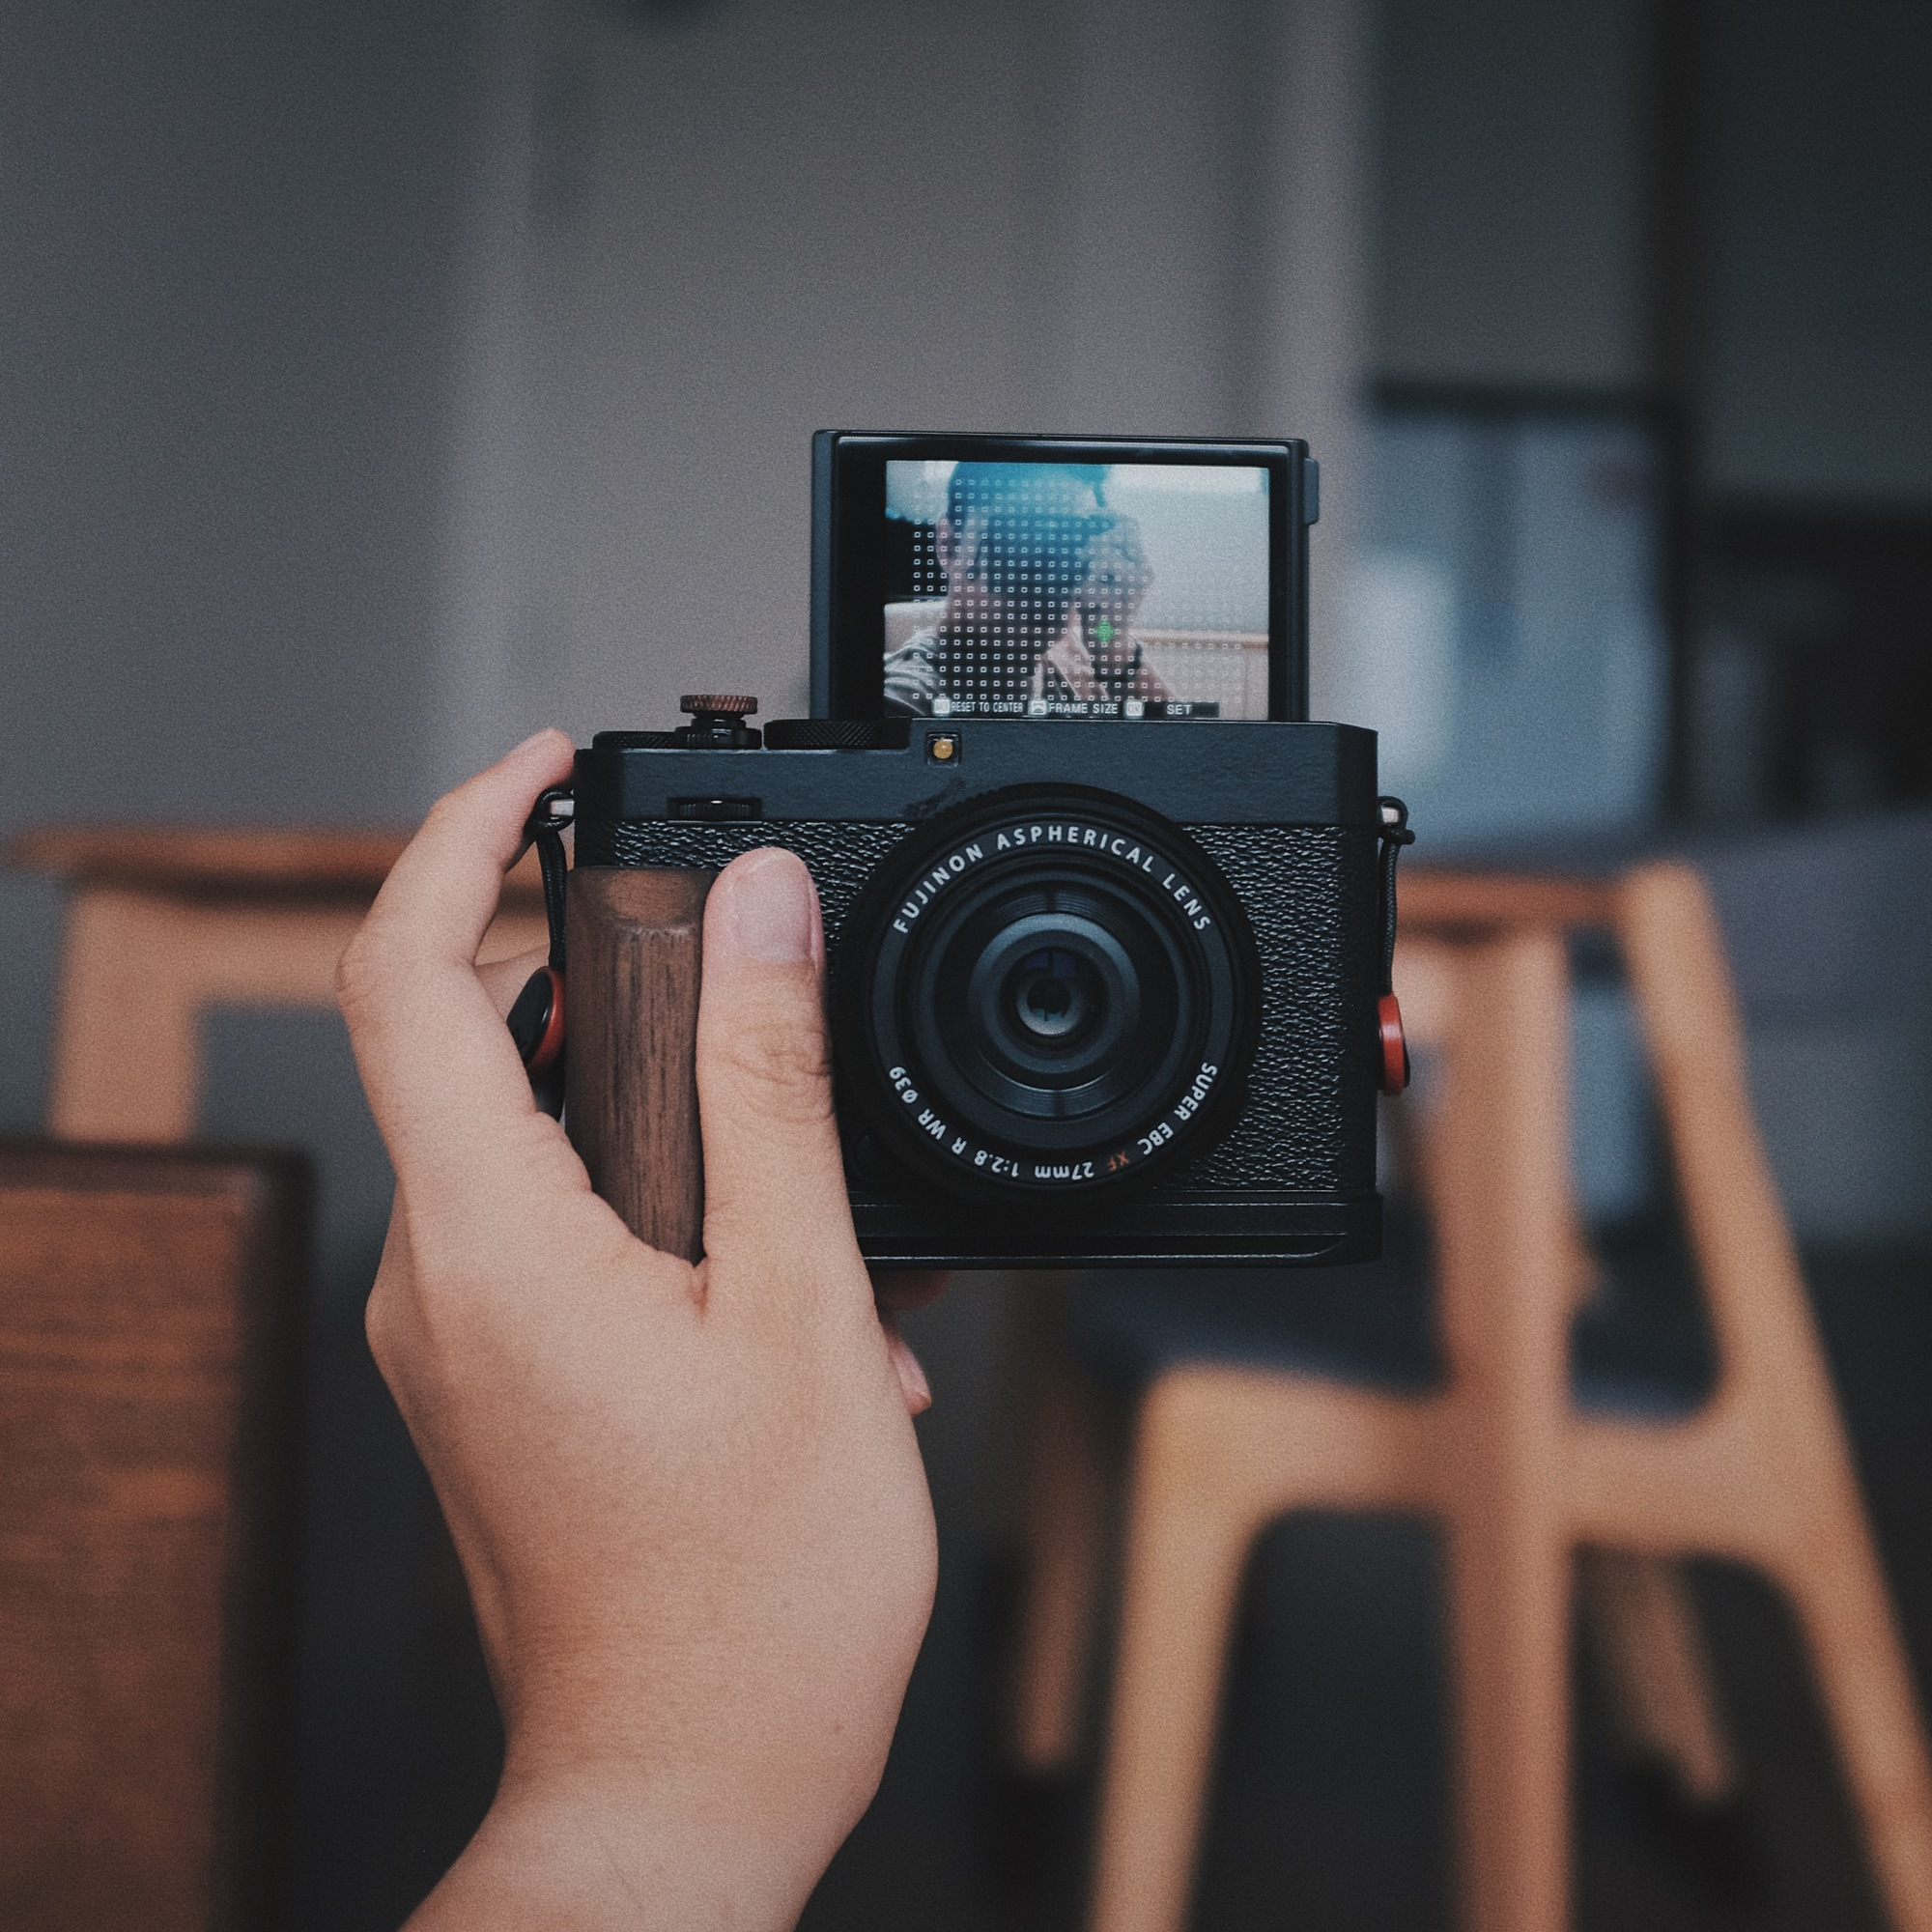
\includegraphics[width=\linewidth]{\envfinaldir/coverpic-prod.jpg}\par
            % \vskip 30pt
            \vfill

            \normalsize\rmfamily\scshape
            \copyright{} The Web Digest Project \hfill\large \envdatestr
        \end{center}
    \end{titlepage}
    % \restoregeometry
}
\newcommand{\simplehref}[1]{%
    \textcolor{blue!80!green}{\href{#1}{#1}}%
}
\renewcommand{\contentsname}{\center\Huge\sffamily\bfseries Contents\par\vskip 20pt}
\newcounter{ipartcounter}
\setcounter{ipartcounter}{0}
\newcommand{\ipart}[1]{
    % \vskip 20pt
    \clearpage
    \stepcounter{ipartcounter}
    \phantomsection
    \addcontentsline{toc}{chapter}{#1}
    % \begin{center}
    %     \Huge
    %     \sffamily\bfseries
    %     #1
    % \end{center}
    % \vskip 20pt plus 7pt
}
\newcounter{ichaptercounter}
\setcounter{ichaptercounter}{0}
\newcommand{\ichapter}[1]{
    % \vskip 20pt
    \clearpage
    \stepcounter{ichaptercounter}
    \phantomsection
    \addcontentsline{toc}{section}{\numberline{\arabic{ichaptercounter}}#1}
    \begin{center}
        \Huge
        \sffamily\bfseries
        #1
    \end{center}
    \vskip 20pt plus 7pt
}
\newcommand{\entrytitlefont}[1]{\subsection*{\raggedright\Large\sffamily\bfseries#1}}
\newcommand{\entryitemGeneric}[2]{
    % argv: title, url
    \parbox{\linewidth}{
        \entrytitlefont{#1}\par\vskip 5pt
        \footnotesize\ttfamily\mdseries
        \simplehref{#2}
    }\vskip 11pt plus 11pt minus 1pt
}
\newcommand{\entryitemGithub}[3]{
    % argv: title, url, desc
    \parbox{\linewidth}{
        \entrytitlefont{#1}\par\vskip 5pt
        \footnotesize\ttfamily\mdseries
        \simplehref{#2}\par\vskip 5pt
        \small\rmfamily\mdseries#3
    }\vskip 11pt plus 11pt minus 1pt
}
\newcommand{\entryitemAp}[3]{
    % argv: title, url, desc
    \parbox{\linewidth}{
        \entrytitlefont{#1}\par\vskip 5pt
        \footnotesize\ttfamily\mdseries
        \simplehref{#2}\par\vskip 5pt
        \small\rmfamily\mdseries#3
    }\vskip 11pt plus 11pt minus 1pt
}
\newcommand{\entryitemHackernews}[3]{
    % argv: title, hnurl, rawurl
    % \parbox{\linewidth}{
    %     \entrytitlefont{#1}\par\vskip 5pt
    %     \footnotesize\ttfamily\mdseries
    %     \simplehref{#3}\par
    %     \textcolor{black!50}{\href{#2}{#2}}
    % }\vskip 11pt plus 11pt minus 1pt
    \begin{minipage}{\linewidth}
            \entrytitlefont{#1}\par\vskip 5pt
            \footnotesize\ttfamily\mdseries
            \simplehref{#3}\par
            \textcolor{black!50}{\href{#2}{#2}}
    \end{minipage}\par\vskip 11pt plus 11pt minus 1pt
}







\begin{document}

\makeheader

\tableofcontents\clearpage




\ipart{Developers}
\ichapter{Hacker News}
\entryitemTwoLinks{South Korean regulator accuses DeepSeek of sharing user data with ByteDance}{https://news.ycombinator.com/item?id=43094651}{https://www.bbc.com/news/articles/c4gex0x87g4o}

\entryitemTwoLinks{AWS paywalling select knowledge base articles, requiring Premium Support plan}{https://news.ycombinator.com/item?id=43094467}{https://repost.aws/knowledge-center/eks-api-server-unauthorized-error}

\entryitemTwoLinks{Valve releases Team Fortress 2 game code}{https://news.ycombinator.com/item?id=43094260}{https://github.com/ValveSoftware/source-sdk-2013/commit/0759e2e8e179d5352d81d0d4aaded72c1704b7a9}

\entryitemTwoLinks{My LLM codegen workflow}{https://news.ycombinator.com/item?id=43094006}{https://harper.blog/2025/02/16/my-llm-codegen-workflow-atm/}

\entryitemTwoLinks{Nuclear fusion: WEST beats the world record for plasma duration}{https://news.ycombinator.com/item?id=43093939}{https://www.cea.fr/english/Pages/News/nuclear-fusion-west-beats-the-world-record-for-plasma-duration.aspx}

\entryitemTwoLinks{Moving on from 18F}{https://news.ycombinator.com/item?id=43093859}{https://ethanmarcotte.com/wrote/leaving-18f/}

\entryitemTwoLinks{Pi-hole v6}{https://news.ycombinator.com/item?id=43093328}{https://pi-hole.net/blog/2025/02/18/introducing-pi-hole-v6/}

\entryitemTwoLinks{Among top researchers 10\% publish at unrealistic levels, analysis finds}{https://news.ycombinator.com/item?id=43093155}{https://www.chemistryworld.com/news/among-worlds-top-researchers-10-publish-at-unrealistic-levels-analysis-finds/4020962.article}

\entryitemTwoLinks{Svelte 5 is not JavaScript}{https://news.ycombinator.com/item?id=43091596}{https://hodlbod.npub.pro/post/1739830562159/}

\entryitemTwoLinks{By the end of today, NASA's workforce will be about 10 percent smaller}{https://news.ycombinator.com/item?id=43090862}{https://arstechnica.com/space/2025/02/by-the-end-of-today-nasas-workforce-will-be-about-10-percent-smaller/}

\entryitemTwoLinks{Tariffs result in 10\% laptop price hike in U.S. says Acer CEO}{https://news.ycombinator.com/item?id=43090684}{https://www.tomshardware.com/laptops/acer-ceo-10pc-price-rise-tariffs}

\entryitemTwoLinks{Show HN: Scripton – Python IDE with built-in realtime visualizations}{https://news.ycombinator.com/item?id=43090214}{https://scripton.dev}

\entryitemTwoLinks{The ideal candidate will be punched in the stomach}{https://news.ycombinator.com/item?id=43089150}{https://www.scottsmitelli.com/articles/ideal-candidate/}

\entryitemTwoLinks{Tesla was hit by a wave of protests, sales are crashing, insiders are waking up}{https://news.ycombinator.com/item?id=43088993}{https://electrek.co/2025/02/17/tesla-was-hit-by-a-wave-of-protests-over-musk-sales-are-crashing-insiders-are-waking-up/}

\entryitemTwoLinks{India's Tata Consultancy Was Gaming the US Visa System}{https://news.ycombinator.com/item?id=43088906}{https://www.bloomberg.com/news/features/2025-02-17/india-s-tcs-misclassified-managers-to-skirt-h-1b-rules-former-staffers-say}

\entryitemTwoLinks{Reviewing the cryptography used by Signal}{https://news.ycombinator.com/item?id=43088785}{https://soatok.blog/2025/02/18/reviewing-the-cryptography-used-by-signal/}

\entryitemTwoLinks{Linux's Sole Wireless/WiFi Driver Maintainer Is Stepping Down}{https://news.ycombinator.com/item?id=43088486}{https://www.phoronix.com/news/Linux-Wireless-Maintainer-2025}

\entryitemTwoLinks{XOR}{https://news.ycombinator.com/item?id=43087944}{https://www.chiark.greenend.org.uk/~sgtatham/quasiblog/xor/}

\entryitemTwoLinks{Show HN: Live-updating version of the 'What a week, huh?' meme}{https://news.ycombinator.com/item?id=43086479}{https://tintin.dlazaro.ca/}

\entryitemTwoLinks{Go 1.24}{https://news.ycombinator.com/item?id=43086170}{https://tip.golang.org/doc/go1.24}\ichapter{Phoronix}
\entryitemGeneric{\hskip 0pt{}NVIDIA GeForce RTX 5080/5090 Performance With Neat Video 6 On Linux}{https://www.phoronix.com/review/nvidia-neat-video-6}

\entryitemGeneric{\hskip 0pt{}Linus Torvalds Would Reportedly Merge Rust Kernel Code Over Maintainer Objections}{https://www.phoronix.com/news/Torvalds-Override-On-Rust-Code}

\entryitemGeneric{\hskip 0pt{}Wasmer 6.0 Wires Up Support For Multiple Heterogeneous Backends}{https://www.phoronix.com/news/Wasmer-6.0-Alpha-1}

\entryitemGeneric{\hskip 0pt{}KDE Plasma 6.3.1 Released With A Few Dozen Fixes For The Week}{https://www.phoronix.com/news/KDE-Plasma-6.3.1-Released}

\entryitemGeneric{\hskip 0pt{}Ubuntu Linux LTS Releases May Offer Additional Intel Graphics Driver Updates}{https://www.phoronix.com/news/Ubuntu-LTS-HWE-More-Intel}

\entryitemGeneric{\hskip 0pt{}AMD Continues Preparing openSIL Concept For Phoenix \& Turin Processors}{https://www.phoronix.com/news/AMD-openSIL-Turin-2025-Coming}

\entryitemGeneric{\hskip 0pt{}openSUSE Spin Achieves 100\% Bit-Identical Packages For Reproducible Builds}{https://www.phoronix.com/news/openSUSE-Reproducible-Build-RB}

\entryitemGeneric{\hskip 0pt{}PostgreSQL Lands Self-Join Elimination Optimization}{https://www.phoronix.com/news/PostgreSQL-Self-Join-Eliminate}

\entryitemGeneric{\hskip 0pt{}SDL \& MPV Media Player Land Support For Wayland Color Management / HDR}{https://www.phoronix.com/news/MPV-SDL-Land-Wayland-Color-HDR}\ichapter{Dribbble}
\entryitemGeneric{\hskip 0pt{}E + Chart Logo Animation}{https://dribbble.com/shots/25640702-E-Chart-Logo-Animation}

\entryitemGeneric{\hskip 0pt{}Reign - Logotype Design}{https://dribbble.com/shots/25639247-Reign-Logotype-Design}

\entryitemGeneric{\hskip 0pt{}Pigeon}{https://dribbble.com/shots/25641861-Pigeon}

\entryitemGeneric{\hskip 0pt{}Oh Baby!!}{https://dribbble.com/shots/25630659-Oh-Baby}

\entryitemGeneric{\hskip 0pt{}Alpaca}{https://dribbble.com/shots/25627851-Alpaca}

\entryitemGeneric{\hskip 0pt{}Cupid}{https://dribbble.com/shots/25629698-Cupid}

\entryitemGeneric{\hskip 0pt{}Happy Valentine's Day}{https://dribbble.com/shots/25629557-Happy-Valentine-s-Day}

\entryitemGeneric{\hskip 0pt{}KOVEX - Logo Design}{https://dribbble.com/shots/25630984-KOVEX-Logo-Design}

\entryitemGeneric{\hskip 0pt{}Flows Lab UX/UI design}{https://dribbble.com/shots/25629797-Flows-Lab-UX-UI-design}

\entryitemGeneric{\hskip 0pt{}Ethereum Wordmark Logo Concept}{https://dribbble.com/shots/25623390-Ethereum-Wordmark-Logo-Concept}

\entryitemGeneric{\hskip 0pt{}IMMO UNIT logo}{https://dribbble.com/shots/25624233-IMMO-UNIT-logo}

\entryitemGeneric{\hskip 0pt{}Illustration}{https://dribbble.com/shots/25619766-Illustration}

\entryitemGeneric{\hskip 0pt{}Carbon Solutions B2B Dashboard Design}{https://dribbble.com/shots/25554521-Carbon-Solutions-B2B-Dashboard-Design}

\entryitemGeneric{\hskip 0pt{}Love Potion}{https://dribbble.com/shots/25619714-Love-Potion}

\entryitemGeneric{\hskip 0pt{}Mortar\&Carrot}{https://dribbble.com/shots/25619708-Mortar-Carrot}

\entryitemGeneric{\hskip 0pt{}Pirate Parrot}{https://dribbble.com/shots/25619077-Pirate-Parrot}

\entryitemGeneric{\hskip 0pt{}SPROXX - LOGO DESIGN}{https://dribbble.com/shots/25619328-SPROXX-LOGO-DESIGN}

\entryitemGeneric{\hskip 0pt{}Master / God / Cloud}{https://dribbble.com/shots/25619810-Master-God-Cloud}

\entryitemGeneric{\hskip 0pt{}Sidebar Quick Actions: Integrations}{https://dribbble.com/shots/25618236-Sidebar-Quick-Actions-Integrations}

\entryitemGeneric{\hskip 0pt{}Fast Turn Fittings}{https://dribbble.com/shots/25619395-Fast-Turn-Fittings}

\entryitemGeneric{\hskip 0pt{}Wolverine Print}{https://dribbble.com/shots/25615908-Wolverine-Print}

\entryitemGeneric{\hskip 0pt{}Cover illustration for Oxford University Press}{https://dribbble.com/shots/25618461-Cover-illustration-for-Oxford-University-Press}

\entryitemGeneric{\hskip 0pt{}Marketing Website Design}{https://dribbble.com/shots/25618155-Marketing-Website-Design}

\entryitemGeneric{\hskip 0pt{}Dirt Construction Site}{https://dribbble.com/shots/25618132-Dirt-Construction-Site}


\ipart{Developers~~~~(zh-Hans)}
\ichapter{Solidot}
\entryitemGeneric{\hskip 0pt{}美国白领工人的工作面临风险}{https://www.solidot.org/story?sid=80583}

\entryitemGeneric{\hskip 0pt{}为什么吃饱之后仍然想吃甜食}{https://www.solidot.org/story?sid=80582}

\entryitemGeneric{\hskip 0pt{}OpenSUSE Tumbleweed 使用的 MAC 切换到 SELinux}{https://www.solidot.org/story?sid=80581}

\entryitemGeneric{\hskip 0pt{}青少年可能不适合断食}{https://www.solidot.org/story?sid=80580}

\entryitemGeneric{\hskip 0pt{}日本政府将重新发展核电}{https://www.solidot.org/story?sid=80579}

\entryitemGeneric{\hskip 0pt{}特朗普政府封禁了 Julianne Moore 的儿童书《Freckleface Strawberry》}{https://www.solidot.org/story?sid=80578}

\entryitemGeneric{\hskip 0pt{}X 屏蔽 Signal.me 链接}{https://www.solidot.org/story?sid=80577}

\entryitemGeneric{\hskip 0pt{}研究认为人类可能并不孤单}{https://www.solidot.org/story?sid=80576}

\entryitemGeneric{\hskip 0pt{}人类的思维在衰退}{https://www.solidot.org/story?sid=80575}

\entryitemGeneric{\hskip 0pt{}韩国应用商店暂停 DeepSeek 下载}{https://www.solidot.org/story?sid=80574}

\entryitemGeneric{\hskip 0pt{}科学家首次观察到水的第四形态}{https://www.solidot.org/story?sid=80573}

\entryitemGeneric{\hskip 0pt{}百度宣布将开源其文心大模型4.5}{https://www.solidot.org/story?sid=80572}

\entryitemGeneric{\hskip 0pt{}Google 允许广告商收集指纹识别数据}{https://www.solidot.org/story?sid=80571}

\entryitemGeneric{\hskip 0pt{}ChatGPT 允许生成成人级内容}{https://www.solidot.org/story?sid=80570}

\entryitemGeneric{\hskip 0pt{}窃取机密的黑客兼职勒索软件攻击者}{https://www.solidot.org/story?sid=80569}

\entryitemGeneric{\hskip 0pt{}世界海冰面积再创新低}{https://www.solidot.org/story?sid=80568}\ichapter{V2EX}
\entryitemGeneric{\hskip 0pt{}[分享创造] [送 40 兑换码] 一个 iOS 的数码物品管理工具}{https://www.v2ex.com/t/1112474}

\entryitemGeneric{\hskip 0pt{}[iCloud] 想问一下时间机器怎么备份 iCloud Drive 的文件}{https://www.v2ex.com/t/1112472}

\entryitemGeneric{\hskip 0pt{}[问与答] 大家觉得现在 ai 算是普及了么}{https://www.v2ex.com/t/1112471}

\entryitemGeneric{\hskip 0pt{}[物联网] 似乎 米家/绿米 的 Zigbee 设备低电量通知从来没生效过!}{https://www.v2ex.com/t/1112470}

\entryitemGeneric{\hskip 0pt{}[PHP] PHP 语言已经过气了吗}{https://www.v2ex.com/t/1112469}

\entryitemGeneric{\hskip 0pt{}[问与答] 115 扩容有什么好推荐?}{https://www.v2ex.com/t/1112468}

\entryitemGeneric{\hskip 0pt{}[宽带症候群] Win11 开 SMB, Mac 和投影仪看 4K UHD 卡}{https://www.v2ex.com/t/1112467}

\entryitemGeneric{\hskip 0pt{}[分享创造] [WeClipper] 剪切板助手 v0.4.5,更加准确的输入光标位置检测来了!}{https://www.v2ex.com/t/1112466}

\entryitemGeneric{\hskip 0pt{}[职场话题] 劳动仲裁后续}{https://www.v2ex.com/t/1112464}

\entryitemGeneric{\hskip 0pt{}[耳机] 馒头真无线 4 和 WF-1000XM5 求推荐}{https://www.v2ex.com/t/1112463}

\entryitemGeneric{\hskip 0pt{}[Apple TV] 再开一贴 讨论一下市面上哪些电视支持完整 CEC 和 QMS}{https://www.v2ex.com/t/1112460}

\entryitemGeneric{\hskip 0pt{}[分享创造] Color Block Jam}{https://www.v2ex.com/t/1112459}

\entryitemGeneric{\hskip 0pt{}[macOS] 15.3.1 GPU 工作较重时外接鼠标会卡顿,触摸板不卡}{https://www.v2ex.com/t/1112458}

\entryitemGeneric{\hskip 0pt{}[问与答] win11 自带录音机 / Microsoft Store 无法更新 如何解决?}{https://www.v2ex.com/t/1112457}

\entryitemGeneric{\hskip 0pt{}[Windows] 微软即将推出官方 PC 迁移助手应用}{https://www.v2ex.com/t/1112456}

\entryitemGeneric{\hskip 0pt{}[问与答] 请教一个 react native FlatList 的问题}{https://www.v2ex.com/t/1112454}

\entryitemGeneric{\hskip 0pt{}[投资] 为啥我在支付宝里买的纳斯达克今天是负数?}{https://www.v2ex.com/t/1112453}

\entryitemGeneric{\hskip 0pt{}[程序员] 电商后端那个方向更好\&区别?商品?交易?营销?履约?还是其他?}{https://www.v2ex.com/t/1112450}

\entryitemGeneric{\hskip 0pt{}[程序员] 监控有什么比较轻量的方案}{https://www.v2ex.com/t/1112449}

\entryitemGeneric{\hskip 0pt{}[分享发现] Grok API 送\$150 刀}{https://www.v2ex.com/t/1112448}

\entryitemGeneric{\hskip 0pt{}[问与答] 台式机配好后网速慢,是网卡的锅,还是天线的锅?}{https://www.v2ex.com/t/1112447}

\entryitemGeneric{\hskip 0pt{}[问与答] B 站来钱最快的视频区——卖肉 评测?}{https://www.v2ex.com/t/1112446}

\entryitemGeneric{\hskip 0pt{}[MacBook Pro] 求推荐一个 MBP 扩展的显示器。}{https://www.v2ex.com/t/1112445}

\entryitemGeneric{\hskip 0pt{}[推广] 广东联通大流量卡 办理年龄仅限 18-30 岁}{https://www.v2ex.com/t/1112444}

\entryitemGeneric{\hskip 0pt{}[问与答] 谷歌地球 PC 版的路网位置都向东偏移了 500+米左右,有没有好的方法解决}{https://www.v2ex.com/t/1112443}

\entryitemGeneric{\hskip 0pt{}[问与答] 有什么好用的在线 提取 抖音链接视频 字幕的网站吗?}{https://www.v2ex.com/t/1112442}

\entryitemGeneric{\hskip 0pt{}[站长] 一个全新的宝宝起名网站!}{https://www.v2ex.com/t/1112440}

\entryitemGeneric{\hskip 0pt{}[全球工单系统] 这年头 3 万 5 一个车位,值得买吗?}{https://www.v2ex.com/t/1112439}

\entryitemGeneric{\hskip 0pt{}[信息安全] 用代理上财新,有什么信息安全的风险不?}{https://www.v2ex.com/t/1112438}

\entryitemGeneric{\hskip 0pt{}[分享发现] 搜狗输入法居然塞进去了一个 PDF 工具,是时候完全转向 Rime 了}{https://www.v2ex.com/t/1112437}

\entryitemGeneric{\hskip 0pt{}[求职] [北京]5 年 Python 后端 想找个工作,求大佬捞}{https://www.v2ex.com/t/1112436}

\entryitemGeneric{\hskip 0pt{}[酷工作] [招聘] nodejs 后端开发工程师}{https://www.v2ex.com/t/1112434}

\entryitemGeneric{\hskip 0pt{}[硬件] anker 到底怎么样}{https://www.v2ex.com/t/1112433}

\entryitemGeneric{\hskip 0pt{}[Java] 有什么好用的可以生成测试用的复杂假数据的软件么?}{https://www.v2ex.com/t/1112432}

\entryitemGeneric{\hskip 0pt{}[问与答] 大家有在 macOS 上用过 loon 吗? 想请问一下体验如何}{https://www.v2ex.com/t/1112431}

\entryitemGeneric{\hskip 0pt{}[问与答] 还有哪些类似 open-webui 的产品?}{https://www.v2ex.com/t/1112430}

\entryitemGeneric{\hskip 0pt{}[Linux] 请教一下 Linux 环境下如何将 word 高保真的转为 pdf}{https://www.v2ex.com/t/1112429}

\entryitemGeneric{\hskip 0pt{}[反馈] 建议将 openAI 节点改名}{https://www.v2ex.com/t/1112428}

\entryitemGeneric{\hskip 0pt{}[职场话题] 来 V2EX 求点建议}{https://www.v2ex.com/t/1112427}

\entryitemGeneric{\hskip 0pt{}[宽带症候群] 运营商真想赚钱增加收入}{https://www.v2ex.com/t/1112426}

\entryitemGeneric{\hskip 0pt{}[Android] 安卓的微信来消息是怎么推送的?}{https://www.v2ex.com/t/1112425}

\entryitemGeneric{\hskip 0pt{}[iPhone] iPhone 的电源键回弹出问题了如何解决?}{https://www.v2ex.com/t/1112424}

\entryitemGeneric{\hskip 0pt{}[天黑以后] 20250218 午夜俱乐部}{https://www.v2ex.com/t/1112423}

\entryitemGeneric{\hskip 0pt{}[问与答] 买电瓶车,坐标广州,求推荐,注重安全和实用}{https://www.v2ex.com/t/1112422}

\entryitemGeneric{\hskip 0pt{}[酷工作] [招聘] 后端开发(郑州/西安)非外包}{https://www.v2ex.com/t/1112421}

\entryitemGeneric{\hskip 0pt{}[问与答] 组电脑想买全塔服务器机箱,有什么需要注意的吗?}{https://www.v2ex.com/t/1112420}

\entryitemGeneric{\hskip 0pt{}[酷工作] [上海] [鹰角] 招聘一个游戏服务端}{https://www.v2ex.com/t/1112419}

\entryitemGeneric{\hskip 0pt{}[酷工作] 快手电商杭州/北京两地招聘前端,快来}{https://www.v2ex.com/t/1112417}

\entryitemGeneric{\hskip 0pt{}[分享创造] rime\_clinic 医学输入法词库项目}{https://www.v2ex.com/t/1112416}

\entryitemGeneric{\hskip 0pt{}[程序员] 大佬们, web 前端面试如何速通 android 与 ios 开发}{https://www.v2ex.com/t/1112415}


\ipart{Generic News}
\ichapter{AP News}
\entryitemWithDescription{\hskip 0pt{}Meghan, the Duchess of Sussex, unveils new lifestyles brand As Ever}{https://apnews.com/article/abdbbf3f6494124d79464843697408d8}{}

\entryitemWithDescription{\hskip 0pt{}Woman sues fertility clinic, saying she gave birth to another patient's baby}{https://apnews.com/article/97190518b80b0805494fc4897c477073}{}

\entryitemWithDescription{\hskip 0pt{}From farms to bakeries, egg shortages and price hikes are challenging small businesses}{https://apnews.com/article/bab4d891b90d2c346629aeeb7a7a81c7}{}

\entryitemWithDescription{\hskip 0pt{}`Saturday Night Live' will next feature Lady Gaga, Shane Gillis and Tate McRae}{https://apnews.com/article/bfb0fc28d3b78f3fb6633634b7c2ce4b}{}

\entryitemWithDescription{\hskip 0pt{}A treasured Banksy owned by a member of Blink-182 is up for auction. It could fetch \$6 million}{https://apnews.com/article/744e225d8d4f6eb344687843309d3fe8}{}

\entryitemWithDescription{\hskip 0pt{}Death of South Korean actor at 24 sparks discussion about social media and internet culture}{https://apnews.com/article/a2ce58f4d63b423afb328709027429ba}{}

\entryitemWithDescription{\hskip 0pt{}Congratulations, March 2 is your day: A free book giveaway honors Dr. Seuss' birthday}{https://apnews.com/article/888556f6b476d1829fa1c3f9fe7a9400}{}

\entryitemWithDescription{\hskip 0pt{}Mexican musical legend Paquita la del Barrio dies at 77}{https://apnews.com/article/67968889ab17bee5751a368a94977d7f}{}

\entryitemWithDescription{\hskip 0pt{}A majority of tennis players have lost faith in doping agencies after Sinner's case, Djokovic says}{https://apnews.com/article/3407d7dc8b961ae3962fec4f5055a864}{}

\entryitemWithDescription{\hskip 0pt{}Shakira resumes world tour with concert in Peru after canceling show due to illness}{https://apnews.com/article/c505c1af1c59aedf12c4072791ef169e}{}

\entryitemWithDescription{\hskip 0pt{}`Saturday Night Live' 50th anniversary special watched by nearly 15 million people}{https://apnews.com/article/82e6424ff69d9ba175cffd195760630a}{}

\entryitemWithDescription{\hskip 0pt{}William Byron avoids late wrecks to win 2nd straight Daytona 500 for Hendrick Motorsports}{https://apnews.com/article/50075048856e22115248a6d802c76ac4}{}

\entryitemWithDescription{\hskip 0pt{}Suspect in Tupac Shakur killing seeks to delay trial as defense identifies new witnesses}{https://apnews.com/article/5e61153292d7e1bd1fe65aa069ed7b40}{}\ichapter{联合早报}
\entryitemWithDescription{沈泽玮:台湾冲突阻遏法案只叫不咬?}{https://www.zaobao.com/news/china/story20240918-4758889}{美国众议院9月9日开启了长达一星期的``中国周'',共通过25项主要涉华法案。(法新社) 美国众议院在当地时间9月9日开启了长达一星期的``中国周'',在美国总统和国会选举举行之前,密集表决数十项与中国有关的法案,共通过25项主要涉华法案……}

\entryitemWithDescription{欧盟电动车关税投票倒计时 中国在分歧中寻支持}{https://www.zaobao.com/news/china/story20240917-4758953}{欧盟27个成员国将于9月25日就是否继续对进口自中国的电动汽车额外征税进行最后表决。图为上海港等待装运出口的电动汽车。(彭博社) 欧盟对中国电动汽车加征关税的投票进入倒计时,正在欧洲访问的中国商务部部长王文涛与欧盟多国政府高层就此进行协商,试图在立场分歧的成员国中争取到更多支持。 受访学者研判,欧盟对中国电动汽车加征关税不可避免,但具体的加税方式和幅度仍有一定弹性,这是王文涛此行与各国谈判的重点……}

\entryitemWithDescription{港府今年将举办逾400项国庆活动}{https://www.zaobao.com/news/china/story20240917-4759341}{再过十多天就是中国国庆75周年,香港天星小轮展示``国庆75周年''\,``三天免费搭小轮''等标语迎国庆。(中新社) 再过十多天就是中国国庆75周年,香港特区政府今年将举办逾400项庆祝活动,希望通过一连串活动庆祝国庆,并且弘扬爱国主义教育及刺激消费。 港府星期二(9月17日)召开记者会,介绍各项庆祝国庆活动和特别优惠,涉及出行及吃喝玩乐等领域……}

\entryitemWithDescription{美空军部长:中国大陆军演精密化 为入侵封锁台湾做准备}{https://www.zaobao.com/news/china/story20240917-4759407}{美国空军部长肯德尔星期一(9月16日)在空军暨太空军协会的一场大会上致辞,提到中国对印太地区日益增长的威胁。(取自美国国防部网站) (华盛顿综合讯)美国空军部长肯德尔指,中国大陆军演的规模越来越大,也更加精密化,这是在专门为入侵、封锁台湾做准备。他也称,中国对印太地区的威胁现在已存在……}

\entryitemWithDescription{批准潜在对台备件军售案后 美派巡逻机过航台海}{https://www.zaobao.com/news/china/story20240917-4758770}{台军士兵8月26日在屏东县枋山训练场进行实弹演习时,从M1167 TOW运载车上发射一枚美制TOW-2A线导反坦克导弹。(路透社) (华盛顿/台北/北京综合讯)在批准潜在对台备件军售案之后,美国派遣反潜巡逻机过航台湾海峡,中国人民解放军东部战区则组织战机跟监美机,并誓言``坚决捍卫国家主权''……}

\entryitemWithDescription{李家超:若香港驻美经贸办被关 受害的是美企}{https://www.zaobao.com/news/china/story20240917-4758797}{香港特首李家超星期一(9月17日)警告,如果美国通过法案,导致香港驻美经贸办关闭,受害的是美国企业。图为李家超9月11日在``一带一路''高峰论坛上致辞。(彭博社) (香港综合讯)香港特首李家超警告,如果美国通过法案,导致香港驻美经贸办关闭,受害的是美国企业。 美国众议院上周通过《香港经济贸易办事处认证法案》,如果参议院也表决通过并交由总统签署成法,香港三个驻美国的经贸办可能将被强制关闭……}

\entryitemWithDescription{美国指中国航空工业集团员工企图实施黑客攻击}{https://www.zaobao.com/news/china/story20240917-4757988}{(华盛顿综合讯)中国航空航天巨头中国航空工业集团一名员工被指试图对美国宇航局、美国军方和其他目标展开黑客攻击。 据彭博社报道,美国检察官布坎南星期一(9月16日)在起诉书中,指控中国航空工业集团39岁的工程师吴宋(音译,Song Wu)企图从美国宇航局、空军、陆军和海军,以及联邦航空管理局取得电脑软件和源代码……}

\entryitemWithDescription{【东谈西论】恒大账务造假 普华永道是共犯还是被拖累?}{https://www.zaobao.com/news/china/story20240917-4756452}{因涉及恒大地产审计项目的违法行为,普华永道中国9月13日被中国财政部和证监会处以4.41亿人民币罚款并被令停业六个月, 广州分所被撤销……}

\entryitemWithDescription{戴庆成:香港输入人才计划大检阅}{https://www.zaobao.com/news/china/story20240917-4744978}{香港于2022年底推出高端人才通行证计划。(法新社) 2019年香港反修例风波过后,数以十万计港人移居海外,令香港出现人才荒。港府为了解决这个问题,在过去几年积极引入``新血'',当中以高才通计划最受瞩目,社会上也不时热议其成效。 高才通全称为高端人才通行证计划,于2022年底推出,申请人年收入须达到250万港元(约42万新元)以上,或本科毕业于全球百强大学并满足一定工作年限等……}

\entryitemWithDescription{中美希望稳定双边关系 中小国家可​​​搭建桥梁}{https://www.zaobao.com/news/china/story20240917-4745091}{中美元首去年11月在旧金山会晤后,双方都希望稳定两国关系,我国巡回大使陈庆珠认为,如果中美两国都认为走向战争不符合它们的利益,那么中小国家就可以做点什么,为双方搭建桥梁。 陈庆珠星期一(9月16日)在李光耀公共政策学院的一场研讨会上说,中国与西方的关系面对诸多困难,有中国智库表示,希望新加坡能协助在中美之间建立更多对话,``因为新加坡受美国信任,也在中国有渠道''……}

\entryitemWithDescription{陈庆珠:世界经历了三次``中国冲击'' 中美的主导力之争将继续}{https://www.zaobao.com/news/china/story20240917-4744996}{李光耀公共政策学院``思想之节庆''的一场研讨会,讨论``历史终结时的中国冲击''。左起是我国巡回大使陈庆珠、通商中国主席李奕贤、李光耀公共政策学院国际关系助理教授何莉菁、李光耀公共政策学院院长柯成兴……}

\entryitemWithDescription{上海遭遇75年来最强台风 扰乱民众中秋假期出行}{https://www.zaobao.com/news/china/story20240916-4745224}{台风贝碧嘉星期一(9月16日)登陆上海,维护人员星期一下午在衡山路上处理倒伏的树木。 (新华社) 台风造成上海上万株数目倒伏或折断。图为一棵倒下的大树砸坏一旁的建筑。(法新社) 台风贝碧嘉登陆上海后,黄浦江苏州河口潮位上涨,乌云密布。(中新社) 中国上海市星期一(9月16日)遭遇75年来最强台风``贝碧嘉''登陆,也是上海有记录以来首次有强台风侵袭……}

\entryitemWithDescription{陆男频长驱偷渡台湾在测试边防实力?}{https://www.zaobao.com/news/china/story20240916-4745161}{中国大陆一名王姓男子在中秋节前夕,乘橡皮艇从浙江宁波抵达台湾新北市林口,主动打电话投案,海巡署人员前去接他上岸。(自由時報) 中国大陆一名王姓男子划橡皮艇于上星期六清晨偷渡到台湾,隔天被新北市地方法院裁定羁押禁见。这是6月以来第二起大陆人士偷渡至台湾,此间专家质疑是否为海防破口,并怀疑对岸是否在测试台湾的边防实力……}

\entryitemWithDescription{中美时隔八月举行国防部工作会晤}{https://www.zaobao.com/news/china/story20240916-4745025}{(北京/华盛顿综合讯)中美双方上周末举行国防部工作会晤;美国官员称,美国积极进行美中两军外交活动,不代表美国对有关中国议题的处理方式发生任何改变。 据中国国防部星期天(15日)晚上通报,北京香山论坛结束后,第18次中美国防部工作会晤上星期六至星期天(9月14日至15日)在北京举行……}

\entryitemWithDescription{中国高校今年拟增足球运动本科专业}{https://www.zaobao.com/news/china/story20240916-4744925}{(北京综合讯)为了培养足球专业人才,中国大专学府今年度拟新增足球运动本科专业,以具体落实中国足球改革。 综合人民网和《南方都市报》报道,中国教育部上星期五(9月13日)发布《2024年度普通高等学校本科专业申报材料公示》。根据公示统计,今年度拟新增专业535个,涉及353所高校,其中39所高校新增足球运动专业……}

\entryitemWithDescription{香港23条首案 港男因穿``光时''上衣被定罪}{https://www.zaobao.com/news/china/story20240916-4743439}{(香港综合讯)香港一名无业男子,今年6月因穿印有2019年反修例抗争口号的上衣而被捕。他星期一承认违反煽动意图罪,成为在《维护国家安全条例》(即《香港基本法》第23条)下被定罪的第一人。 综合港媒《星岛日报》和路透社报道,27岁无业男子诸启邦今年6月12日在石门港铁站附近,未能出示身份证供查阅被警方拘捕……}

\entryitemWithDescription{美国务院:中国释放被关押近20年美籍牧师}{https://www.zaobao.com/news/china/story20240916-4744614}{(华盛顿综合电)中国释放被关押近20年的美国籍牧师,显示北京在中美关系的关键时刻展现善意。 综合彭博社、法新社和路透社报道,美国国务院发言人星期天(9月15日)说:``我们欢迎林大卫(音译,David Lin)从中华人民共和国的监狱获释。他已回返美国,这是他近20年来首次与家人见面。'' 林大卫的女儿艾丽斯告诉美国政治新闻网Politico,她的父亲将抵达得克萨斯州的圣安东尼奥……}

\entryitemWithDescription{中国驻泰使馆:近期并未向湄公河下游泄洪}{https://www.zaobao.com/news/china/story20240916-4743917}{(北京讯)泰国西北部的湄公河因洪水泛滥而决堤,中国否认这是中方泄洪所致,并称近来已持续减少云南景洪水电站的出库流量,以助下游地区抗洪。 中国驻泰国大使馆星期日(9月15日)深夜在官方微信公众号发文说,当天又有媒体报道称中国正在向湄公河泄洪,经向中国主管部门核实,使馆再次澄清,为帮助下游地区应对洪灾,中方近来持续稳定和减少景洪水电站出库流量,不可能对下游地区抗洪救灾形成压力……}

\entryitemWithDescription{加入美国储存可靠度评估计划 台湾军方编列预算采购三类型导弹}{https://www.zaobao.com/news/china/story20240916-4743826}{(台北讯)据台媒报道,台湾军方持续向美国采购可简易操作的导弹,预计在2024年、2031年以前获得400枚``标枪''反装甲导弹、2485枚``刺针''人携式防空导弹……}

\entryitemWithDescription{韩咏红:中美分头追逐全球南方}{https://www.zaobao.com/news/china/story20240916-4730719}{9月5日,中国外长王毅(中)同中非合作论坛非方现任共同主席国塞内加尔外长法勒(左)、下任共同主席国刚果外长加科索(右),在北京共同会见中外记者并答问。(路透社) 进入气候宜人的9月,中国接连举行了两场受瞩目的国际会议,一是聚集非洲53国国家元首与政要的中非合作论坛,接着是周末刚闭幕的北京香山论坛。 两场活动的参与者不同,规模也有很大差距……}

\entryitemWithDescription{菲律宾船只撤离中菲争议海域后 将再派船接替}{https://www.zaobao.com/news/china/story20240915-4730494}{这张在9月15日拍摄,并由菲律宾海岸警卫队提供的照片显示,菲律宾海岸警卫队船马格巴努亚号抵达了菲国巴拉望岛的一个港口。菲律宾早前以发现填海活动为由,今年4月派出马格巴努亚号前往萨比纳礁。(法新社/菲律宾海岸警卫队) 菲律宾国家海事委员会星期天(9月15日)发声明称,该国海岸警卫队一艘巡逻舰已离开萨比纳礁争议海域……}

\entryitemWithDescription{台风贝碧嘉直击中国华东 多趟本地与沪杭间航班取消}{https://www.zaobao.com/news/china/story20240915-4730611}{9月15日在上海外滩滨江步道上,一名外籍游客的雨伞被大风吹起。台风贝碧嘉的中心当天下午5时位于上海市东偏南方大约435公里的东海海面上,中心附近最大风力有13级。(中新社) (上海/新加坡综合讯)台风贝碧嘉预计将为中国华东沿海地区带来狂风暴雨,多趟往返新加坡与上海和杭州的航班取消……}






\clearpage
\leavevmode\vfill
\footnotesize

Copyright \copyright{} 2023-2025 Neruthes and other contributors.

This document is published with CC BY-NC-ND 4.0 license.

The entries listed in this newsletter may be copyrighted by their respective creators.

This newsletter is generated by the Web Digest project.

The newsletters are also delivered via Telegram channel \CJKunderline{\href{https://t.me/webdigestchannel}{https://t.me/webdigestchannel}}.\\
RSS feed is available at \CJKunderline{\href{https://webdigest.pages.dev/rss.xml}{https://webdigest.pages.dev/rss.xml}}.

This newsletter is available in PDF at
\CJKunderline{\href{https://webdigest.pages.dev/}{https://webdigest.pages.dev/}}.

The source code being used to generate this newsletter is available at\\
\CJKunderline{\href{https://github.com/neruthes/webdigest}{https://github.com/neruthes/webdigest}}.

This newsletter is also available in
\CJKunderline{\href{http://webdigest.pages.dev/readhtml/\envyear/WebDigest-20250219.html}{HTML}} and
\CJKunderline{\href{https://github.com/neruthes/webdigest/blob/master/markdown/\envyear/WebDigest-20250219.md}{Markdown}}.


\coverpic{https://unsplash.com/photos/a-close-up-of-a-cell-phone-with-a-blurry-background-cTlimlJPNE4}{Milad Fakurian}


\end{document}
